\documentclass{article}
\usepackage[utf8]{inputenc}
\usepackage[spanish]{babel}
\usepackage{graphicx} % Paquete necesario para cargar archivos de imagen
\usepackage{wrapfig} % Paquete necesario para cargar texto alrededor de imágenes y tablas
\usepackage{lipsum}
\usepackage{subcaption} % Paquete necesario para subfiguras
\usepackage{colortbl} % Paquete para agregar color a tablas
\usepackage{multicol, multirow} % Paquetes para combinar celdas
\usepackage{slashbox}
\usepackage{vmargin} % Paquete para configurar márgenes
\setpapersize{A4}
\setmargins{2.5cm} % margen izquierdo
{1.5cm} % Margen superior
{16.5cm} % Ancho del área de impresión
{23.42cm} % Largo del área de impresión
{10pt} % Espacio de encabezado
{1cm} % Espacio entre encabezado y texto
{0pt} % Espacio de pie de página
{1cm} % Espacio entre el texto y el pie de pagina

\title{Ejemplo uso de imágenes y tablas}
\author{Mg. Fausto Mauricio Lagos Suárez}
\date{Junio 14, 2017}

\usepackage{xcolor}

\definecolor{blue254}{HTML}{25289E}
\definecolor{orange22}{HTML}{E55500}
\definecolor{myBlue}{HTML}{027FDF}
\definecolor{negative}{HTML}{181818}
\definecolor{positive}{HTML}{AA3939} % Paleta de colores
%% -----------------------------------------------------------------------------
%% 2017 por Fausto M. Lagos S. <piratax007@protonmail.ch>
%% 
%% Este trabajo puede ser distribuido o modificado bajo los
%% términos y condiciones de la LaTeX Project Public License (LPPL) v1.3C, 
%% o cualquier versión posterior. La última versión de esta licencia
%% puede verse en:
%% http://www.latex-project.org/lppl.txt
%% 
%% -----------------------------------------------------------------------------
%% Usted es libre de usarlo, modificarlo o distribuirlo siempre que se
%% respeten los términos de la licencia y se reconozca a los autores originales
%% -----------------------------------------------------------------------------
%% Estos comandos y ambientes están desarrollados para el Curso de LaTeX
%% de https://www.youtube.com/c/BrainOnTube y algunos han sido desarrollados
%% por https://github.com/jdleesmiller/latex-course, tenga presente sus
%% nombres y licencia para poder hacer uso de éstos.
%% -----------------------------------------------------------------------------

\usepackage{xkeyval}
\usepackage{minted}
\usepackage{tikz}
\usetikzlibrary{
	calc, angles, quotes, positioning,
    babel, shapes, arrows, shadows
    }
\usepackage{tcolorbox}
\usepackage{xstring}

\newcommand{\bftt}[1]{\textbf{\texttt{#1}}}
\newcommand*\keystroke[1]{%
  \tikz[baseline=(key.base)]
    \node[%
      draw,
      fill=white,
      drop shadow={shadow xshift=0.25ex,shadow yshift=-0.25ex,fill=black,opacity=0.75},
      rectangle,
      rounded corners=2pt,
      inner sep=1pt,
      line width=0.5pt,
      font=\scriptsize\sffamily
    ](key) {#1\strut}
  ;
}
\newcommand{\keystrokebftt}[1]{\keystroke{\bftt{#1}}}
\renewcommand{\comment}[1]{{\color[HTML]{008080}\textit{\textbf{\texttt{#1}}}}}
\newcommand{\cmd}[1]{{\color[HTML]{008000}\bftt{#1}}} % comandos
\newcommand{\bs}{\char`\\}
\newcommand{\cmdbs}[1]{\cmd{\bs#1}}
\newcommand{\lcb}{\char '173}
\newcommand{\rcb}{\char '175}
\newcommand{\cmdbegin}[1]{\cmdbs{begin\lcb}\bftt{#1}\cmd{\rcb}}
\newcommand{\cmdend}[1]{\cmdbs{end\lcb}\bftt{#1}\cmd{\rcb}}
\newcommand{\wllogo}{\textbf{Overleaf}}

\newenvironment{exampletwouptiny}
  {\VerbatimEnvironment
   \begin{VerbatimOut}{example.out}}
  {\end{VerbatimOut}
   \setlength{\parindent}{0pt}
   \fbox{\begin{tabular}{l|l}
   \begin{minipage}{0.55\linewidth}
     \inputminted[fontsize=\scriptsize,resetmargins]{latex}{example.out}
   \end{minipage} &
   \begin{minipage}{0.35\linewidth}
     \setlength{\parskip}{6pt plus 1pt minus 1pt}%
     \raggedright\scriptsize\input{example.out}
   \end{minipage}
   \end{tabular}}}
   
\newenvironment{exampletwouptinynoframe}
  {\VerbatimEnvironment
   \begin{VerbatimOut}{example.out}}
  {\end{VerbatimOut}
   \setlength{\parindent}{0pt}
   \begin{tabular}{l|l}
   \begin{minipage}{0.55\linewidth}
     \inputminted[fontsize=\scriptsize,resetmargins]{latex}{example.out}
   \end{minipage} &
   \begin{minipage}{0.35\linewidth}
     \setlength{\parskip}{6pt plus 1pt minus 1pt}%
     \raggedright\scriptsize\input{example.out}
   \end{minipage}
   \end{tabular}}

\newcommand\diag[4]{%
  \multicolumn{1}{p{#2}|}{\hskip-\tabcolsep
  $\vcenter{\begin{tikzpicture}[baseline=0,anchor=south west,inner sep=#1]
  \path[use as bounding box] (0,0) rectangle (#2+2\tabcolsep,\baselineskip);
  \node[minimum width={#2+2\tabcolsep-\pgflinewidth},
        minimum  height=\baselineskip+\extrarowheight-\pgflinewidth] (box) {};
  \draw[line cap=round] (box.north west) -- (box.south east);
  \node[anchor=south west] at (box.south west) {#3};
  \node[anchor=north east] at (box.north east) {#4};
 \end{tikzpicture}}$\hskip-\tabcolsep}}
 
\newtheorem{definition}{\bf Definición:}

\newtheorem{ejemplo}{\bf Ejemplo:}[section]

\newcounter{remark}
\newenvironment{remark}[1]
{
	\refstepcounter{remark}
	\begin{tcolorbox}[colback = myBlue!25, colframe = firebrick!75, title=\textbf{Observación \theremark: } #1, arc = 3mm, sharp corners = northwest]
	\fontfamily{qag}\selectfont
}
{
	\end{tcolorbox}
}

\newcommand{\Ref}[2]{
	\IfEqCase {#1}{
		{fig}{
			\textbf{Fig. \ref{#2}}
		}
		{tab}{
			\textbf{Tabla. \ref{#2}}
		}
	}
} % Comandos para escritura de código LaTeX
\graphicspath{{./images/}} % Define el directorio de imágenes

\begin{document}
\maketitle
\renewcommand{\tablename}{Tabla}
\renewcommand{\figurename}{Fig.}
\renewcommand{\contentsname}{Tabla de Contenido}
\renewcommand{\listfigurename}{Lista de Figuras}
\renewcommand{\listtablename}{Lista de Tablas}
\tableofcontents % Genera la tabla de contenido de los títulos de secciones y subsecciones
\listoffigures % Genera la lista de figuras
\listoftables % Genera la lista de tablas

\section{Cargar imágenes en un documento \LaTeX{}}

El ambiente \cmd{figure} crea un objeto flotante que estará numerado consecutivamente a lo largo del documento y que por tanto puede ser incluido en la tabla de contenido dentro de la lista de figuras con el comando \cmdbs{listoffigure}.

\begin{figure}[ht]
	\centering
    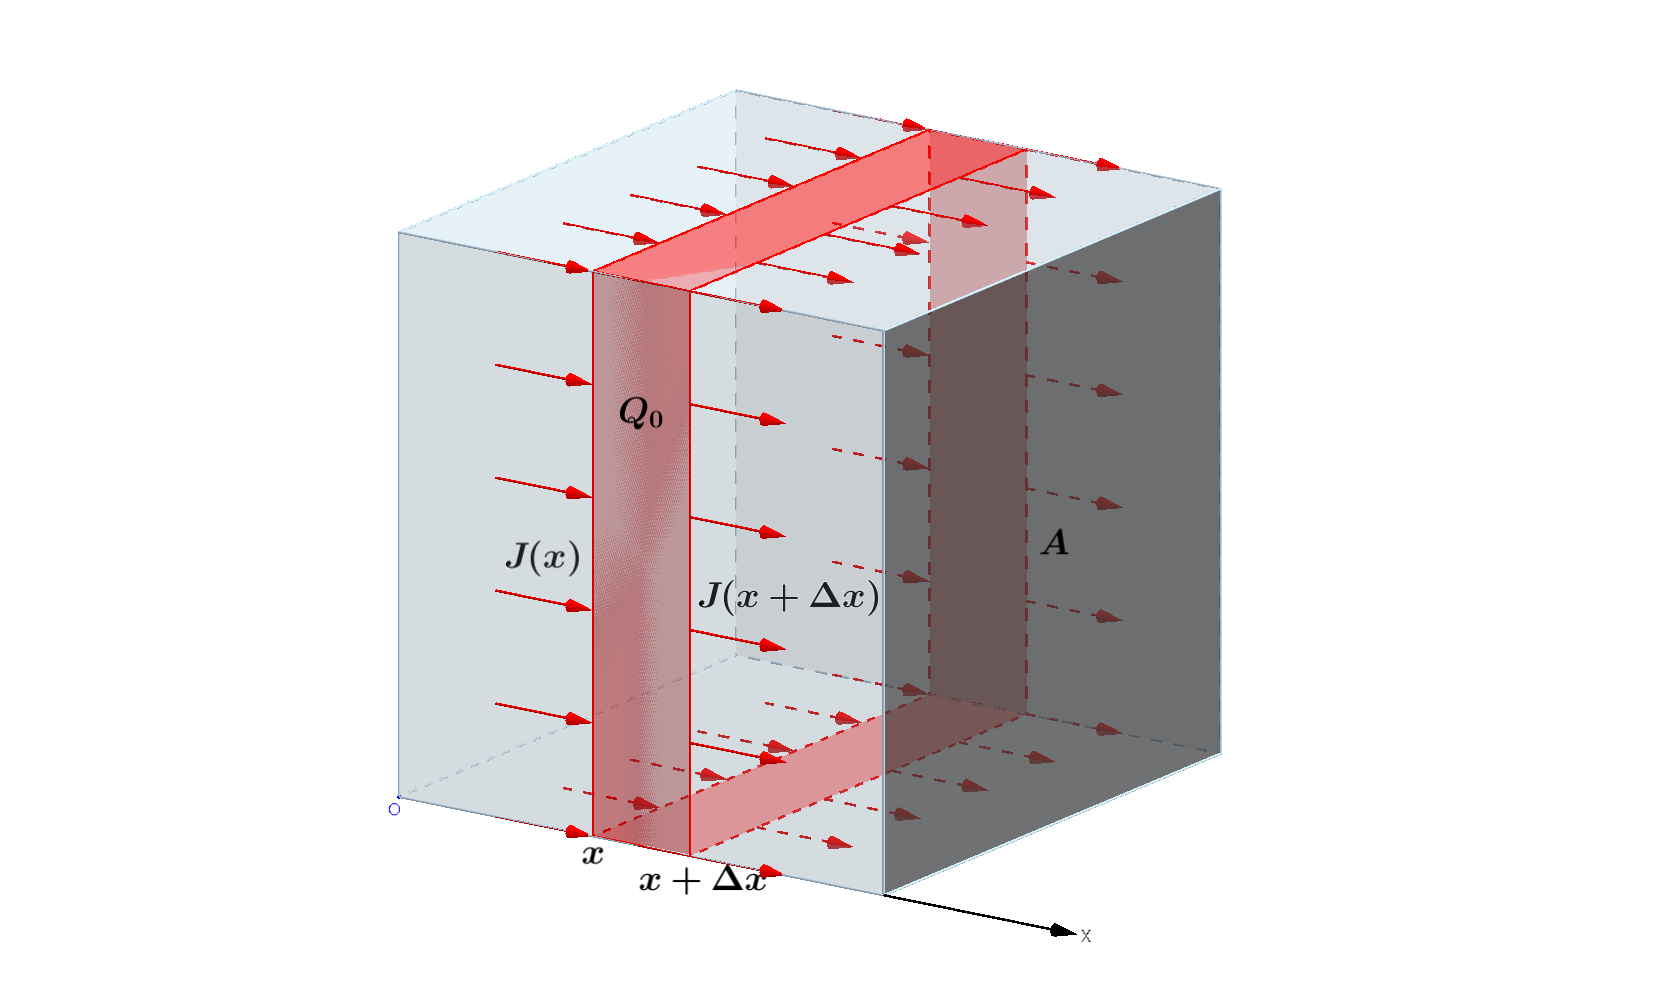
\includegraphics[scale = .4]{cubo}
    \caption{Flujo de temperatura en un cubo}
\end{figure}

El parámetro que define el tamaño de la imagen (\cmd{scale}) puede utilizarse también en unidades de longitud dadas en \bftt{mm, cm, pt, px} con las opciones \bftt{width} y \bftt{height}, por otro lado el \bftt{caption} puede ubicarse antes o después de la imágen (tabla), simplemente el comando \cmdbs{caption} debe escribirse en la posición donde se quiere que aparezca.

\subsection{El paquete \bftt{wrapfig}}

Este paquete, básicamente permite ubicar un objeto flotante (tabla o figura) dentro del texto. El texto circundante a la figura o tabla debe incluirse inmediatamente después de cerrar el ambiente \cmd{wrapfigure}.

\begin{wrapfigure}[12]{L}[5mm]{.45\textwidth}
	\centering
    \caption{Flujo de temperatura en un cilindro}
    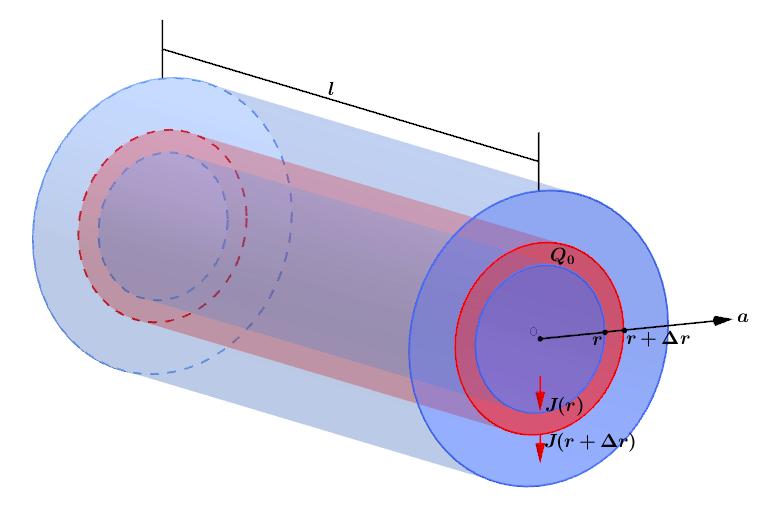
\includegraphics[width = 5cm]{cilindro}
\end{wrapfigure}
\textcolor{gray!95}{\lipsum[1-2]}

\subsection{El paquete \bftt{subcaption}}

Utilizar subfiguras es una herramienta muy útil para algunos documentos \LaTeX{}, el paquete \cmd{wrapfigure} permite hacer esto de manera eficiente y altamente configurable.

\begin{figure}[ht]
	\centering
    \begin{subfigure}[t]{.475\textwidth}
    	\centering
    	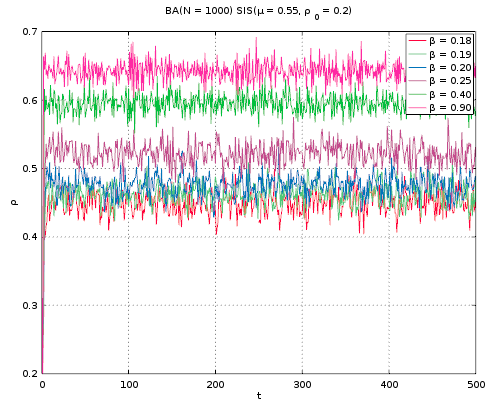
\includegraphics[scale = .45]{BA_1000_u055_p_t_}
        \caption{Dispersión de la gripe}
    \end{subfigure}
    \hfill
    \begin{subfigure}[t]{.45\textwidth}
        \centering
        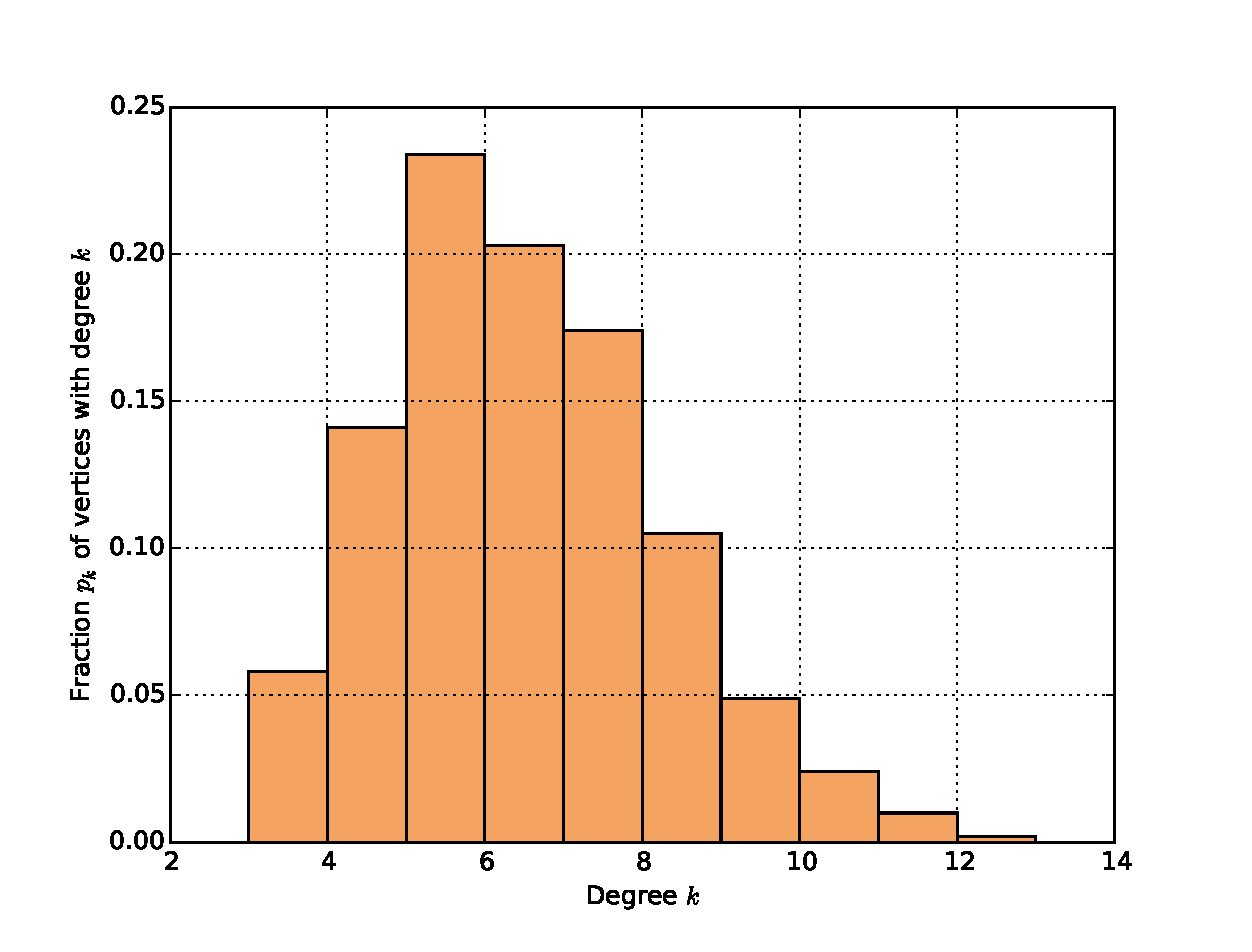
\includegraphics[scale = .35]{histws1000}
        \caption{Clasificación de vértices de acuerdo al grado}
    \end{subfigure}
    \caption{Subfiguras con el paquete \bftt{subcaption}}
\end{figure}

\section{Construcción de tablas simples}

El ambiente \cmd{table} define un objeto flotante \emph{tabla} y el ambiente \cmd{tabular} define el arreglo en filas y columnas, el uso básico del ambiente \cmd{tabular} es idéntico al uso de cualquiera de los ambientes para definición de matrices.

\begin{wraptable}[10]{R}[5mm]{.4\textwidth}
	\centering
    \begin{tabular}{ccc}
    	$\mathbf{x}$ & $\mathbf{y}$ & $\mathbf{f_{xy}(x, y)}$ \\
        \hline
        -1 & -2 & $\frac{1}{8}$ \\
        -0.5 & -1 & $\frac{1}{4}$ \\
        0.5 & 1 & $\frac{1}{2}$ \\
        1 & 2 & $\frac{1}{8}$ \\
        \hline
    \end{tabular}
    \caption{Tabla automática}
\end{wraptable}

\textcolor{gray!95}{\lipsum[1]}

Los comandos \cmdbs{tabcolsep}, \cmdbs{arraystretch} y \cmdbs{arrayrulewidth} intervienen para mejorar el espaciamiento entre el contenido de cada celda de la tabla y los bordes, y el grosor de los bordes de la tabla.

\renewcommand{\tabcolsep}{3mm}
\renewcommand{\arraystretch}{1.5}
\renewcommand{\arrayrulewidth}{1pt}
\begin{table}[ht]
	\centering
    \begin{tabular}{ccc}
    	$\mathbf{x}$ & $\mathbf{y}$ & $\mathbf{f_{xy}(x, y)}$ \\
        \hline
        -1 & -2 & $\frac{1}{8}$ \\
        -0.5 & -1 & $\frac{1}{4}$ \\
        0.5 & 1 & $\frac{1}{2}$ \\
        1 & 2 & $\frac{1}{8}$ \\
        \hline
    \end{tabular}
    \caption{Tabla con separación personalizada}
\end{table}

\begin{wraptable}[13]{L}{.65\textwidth}
	\centering
    \begin{tabular}{|l|c|c|c|}
    	\hline
    	\backslashbox{Adición}{Cesión} & CNC & CNS & CM \\
        \hline \hline
        CNC & & & \\
        \hline
        CNS & & & \\
        \hline
        CM & & & \\
        \hline
    \end{tabular}
    \caption{Tabla con separación diagonal}
\end{wraptable}
Algunas veces es útil dividir en diagonal el contenido de una celda, esta es la función del comando \cmdbs{backslashbox} derivado del paquete \cmd{slashbox} el cual es un paquete muy pequeño cuya única finalidad es hacer este tipo de división por lo tanto no se encuentra instalado en la distribución estándar de \LaTeX{}, puede tenerlo a disposición copiando el archivo \bftt{slashbox.sty} en la carpeta del documento donde lo utilice.

\subsection{Agregar color a las tablas}

El paquete \cmd{colortbl} define comandos para agregar color a filas, columnas y celdas.

\begin{table}[ht]
	\centering
    \begin{tabular}{|l|c|>{\columncolor{emeraldGreen!50}}c|>{\columncolor{myOrange!30}}c|}
    	\hline
        \rowcolor{signBlue!50}
    	\textbf{Clase} & $\mathbf{x_i}$ & $\mathbf{f_i}$ & $\mathbf{h_i}$ \\
        \hline
        $[5, 10)$ & 7.5 & 5 & 0.5 \\
        \hline
        $[10, 15)$ & 12.5 & 8 & 0.24 \\
        \hline
        $[15, 20)$ & 17.5 & 8 & 0.24 \\
        \hline
        $[20, 25)$ & \cellcolor{myRed!75}{22.5} & 10 & 0.39 \\
        \hline
        $[25, 30]$ & 27.5 & 2 & 0.07 \\
        \hline
    \end{tabular}
    \caption{Ejemplo 1 de tabla con colores}
\end{table}

\textcolor{gray!95}{\lipsum[1-2]}

\begin{table}[ht]
	\centering
    \caption{Ejemplo 2 de tabla con colores}
    \rowcolors{1}{darkOliveGreen2!35}{myBlue!35}
    \begin{tabular}{ll}
    	\hline
    	Población empadronada en España & 46.600.949 \\
        Población española & 41.882.085 \\
        Población extranjera & 4.718.864 (10.1 \%) \\
        Población extranjera de 16 años & 16 \% \\
        Población extranjera $< 16$ años & 15.8\% \\
        Países de procedencia más frecuentes & \\
        \begin{tabular}{ll}
        Rumania & 15.9\% \\
        Marruecos & 15.8 \% \\
        China & 4.05\%
        \end{tabular} & \\
        \hline
    \end{tabular}
\end{table}

\subsection{Combinar celdas}

Los paquetes \cmd{multicol} y \cmd{multirow} permiten hacer la combinación de celdas en tablas \LaTeX{}.

\textcolor{gray!95}{\lipsum[1-2]}

\begin{table}[ht]
	\centering
    \begin{tabular}{|>{\cellcolor{myBlue!75}}cc|c|c|}
    	\hline
    	\rowcolor{myBlue!75}
    	& \multicolumn{3}{c|}{\textcolor{white}{Tolerancia Resistiva ($\pm$)}} \\
        \rowcolor{myBlue!75}
        & \textcolor{white}{20\%} & \textcolor{white}{10\%} & \textcolor{white}{5\%} \\
        & \multirow{4}{*}{100} & \multirow{2}{*}{100} & 100 \\ 
        \cline{4-4}
        & & & 91 \\
        \cline{3-4}
        & & \multirow{2}{*}{82} & 82 \\
        \cline{4-4}
        & & & 75 \\
        \cline{2-4}
        & \multirow{4}{*}{68} & \multirow{2}{*}{68} & 68 \\
        \cline{4-4}
        & & & 62 \\
        \cline{3-4}
        & & \multirow{2}{*}{56} & 56 \\
        \cline{4-4}
        & & & 51 \\
        \cline{2-4}
        & \multirow{4}{*}{47} & \multirow{2}{*}{47} & 47 \\
        \cline{4-4}
        & & & 43 \\
        \cline{3-4}
        & & \multirow{2}{*}{39} & 39 \\
        \cline{4-4}
        & & & 36 \\
        \cline{2-4}
        & \multirow{4}{*}{33} & \multirow{2}{*}{33} & 33 \\
        \cline{4-4}
        & & & 30 \\
        \cline{3-4}
        & & \multirow{2}{*}{27} & 27 \\
        \cline{4-4}
        & & & 24 \\
        \cline{2-4}
        & \multirow{4}{*}{22} & \multirow{2}{*}{22} & 22 \\
        \cline{4-4}
        & & & 20 \\
        \cline{3-4}
        & & \multirow{2}{*}{18} & 18 \\
        \cline{4-4}
        & & & 16 \\
        \cline{2-4}
        & \multirow{4}{*}{15} & \multirow{2}{*}{15} & 15 \\
        \cline{4-4}
        & & & 13 \\
        \cline{3-4}
        & & \multirow{2}{*}{12} & 12 \\
        \cline{4-4}
        & & & 11 \\
        \cline{2-4}
        \multirow{-25}{*}{\rotatebox[origin=c]{90}{\textcolor{white}{Valores de Resistencia Estándar}}} & 10 & 10 & 10 \\
        \hline
    \end{tabular}
    \caption{Valores estándar para resistencias con diferente nivel de precisión.}
\end{table}

\end{document}